\section{遇到的问题与解决方法}

本实验在调试过程中遇到了多个问题，以下按发现顺序逐一记录。

\subsection{时序违例}

\textbf{问题}：Vivado实现阶段报告关键路径时序违例，最差负裕量（WNS）为$-5.150$ ns，无法满足时序约束。

\textbf{原因}：系统时钟约束设为100 MHz（10 ns周期），但DDR2 MIG IP核的初始化校准和内部逻辑在较高频率下存在较长的组合路径延迟。

\textbf{解决}：将Clocking Wizard的输出时钟从100 MHz降低到50 MHz（20 ns周期），时序满足要求。

\subsection{SPI Flash控制器未自动启动}

\textbf{问题}：CPU复位后无法从Flash取指，系统无任何响应。

\textbf{原因}：Flash控制器（\texttt{flash\_rom.v}）的IDLE状态中存在\texttt{flash\_continue}门控信号，导致控制器在IDLE状态等待外部启动信号才能发起SPI读取事务。但在本系统架构中，Flash作为CPU的唯一取指来源，CPU第一条指令就必须从Flash获取，不存在外部触发信号。

\textbf{解决}：移除IDLE状态的\texttt{flash\_continue}门控条件，使Flash控制器在收到CPU的Wishbone读请求后自动从IDLE进入START状态发起读取。

\subsection{PLL锁定信号未接入复位}

\textbf{问题}：系统在上电初期偶尔出现不可预期的行为，CPU执行出错。

\textbf{原因}：复位逻辑仅连接板载复位按钮（\texttt{rst\_n}），未考虑Clocking Wizard的PLL锁定状态。在FPGA上电后，PLL需要一定时间完成锁定，此时输出时钟可能不稳定，但复位信号已经释放，导致CPU在时钟不稳定期间执行了错误操作。

\textbf{解决}：将PLL锁定信号\texttt{locked}接入复位逻辑，确保在PLL完成锁定前系统保持复位状态：
\begin{lstlisting}[caption={PLL锁定接入复位}]
assign rst = ~rst_n | ~locked;
\end{lstlisting}

\subsection{DDR2初始化轮询死锁}

\textbf{问题}：系统启动后卡死，数码管无显示，串口无输出。

\textbf{原因}：BootLoader在偏移约\texttt{0x60}处有一个轮询循环，等待GPIO的第16位（即\texttt{sdram\_init\_done}信号）变为1后才开始搬移OS映像。该信号由MIG IP核在校准完成后输出。在正常工作流程中，MIG校准会在数百毫秒内完成。但分析发现，如果GPIO的连接或DDR2初始化存在异常，该轮询将永远无法退出，导致系统死锁。

\textbf{解决}：在SoC顶层（\texttt{openmips\_min\_sopc.v}）中强制将GPIO输入的第16位置1，绕过BootLoader的DDR2就绪轮询：
\begin{lstlisting}[caption={强制绕过DDR2轮询}]
assign gpio_i_temp = {15'h0, 1'b1, gpio_i};
\end{lstlisting}
该修改将\texttt{sdram\_init\_done}信号固定为1，使BootLoader不再等待而直接开始搬移OS映像。由于MIG校准在系统上电后会自动完成且先于CPU执行，该绕过在实际硬件上不会引起问题。

\subsection{SPI Flash采样相位错位（核心问题）}

\textbf{问题}：上述问题逐一解决后，CPU可以取指但执行结果错误——数码管不显示预期内容，串口无输出。通过LED调试探针发现，Flash控制器读取的首条指令高字节为\texttt{0x78}，而期望值为\texttt{0x3C}（指令\texttt{lui \$1, 0x1000}的机器码\texttt{0x3C011000}的最高字节）。\texttt{0x78}恰好是\texttt{0x3C}左移1位的结果。

\textbf{原因分析}：Flash控制器的READ\_DATA状态机使用\texttt{sdo\_count}计数器（0--15循环）来逐位采样SPI数据线\texttt{so}上的数据。原始设计中采用偶数拍（\texttt{sdo\_count}为偶数时）采样、\texttt{sdo\_count == 0}时捕获字节。但通过Vivado ILA（集成逻辑分析仪）抓取实际波形后发现：

\begin{itemize}[leftmargin=2em]
    \item 状态机的\texttt{state}信号比\texttt{sdo\_count}信号慢一拍（\texttt{state}经过两级寄存器更新，\texttt{sdo\_count}只有一级），导致进入READ\_DATA1状态时\texttt{sdo\_count}已经为1而非0。
    \item 第一个数据位（byte0的最高位bit7）出现在\texttt{sdo\_count == 0}的时钟周期，但此时\texttt{state}仍停留在ADDR3\_OUT状态（该状态不发采样），导致该位被漏采。
    \item 后续所有数据位整体偏移1位，每字节左移1位，末位补进下一字节的最高位，最终\texttt{read\_data}等于实际指令左移1位的结果。
\end{itemize}

\textbf{解决}：通过ILA波形精确确认\texttt{datain\_shift}的逐拍演化过程后，将采样相位调整为奇数拍（\texttt{sdo\_count[0]}为1时采样），字节捕获时机调整为\texttt{sdo\_count == 2}。具体修改为：
\begin{lstlisting}[caption={SPI采样相位修正（READ\_DATA2--5的捕获逻辑）}]
// 采样：偶数拍 -> 奇数拍（5处 READ_DATA1-5）
if (sdo_count[0]) begin
    datain_shift <= {datain_shift[6:0], sdi};
end

// 捕获：sdo_count==0 -> sdo_count==2（4处 READ_DATA2-5）
if (sdo_count == 4'd2) begin
    read_data[XX:XX] <= datain_shift;
    datain <= datain_shift;
end
\end{lstlisting}

该修正确保每个数据位在SCK上升沿后的稳定采样点被正确捕获，4字节对齐关系为：byte0在READ\_DATA2的\texttt{sdo\_count == 2}时捕获，byte1在READ\_DATA3的\texttt{sdo\_count == 2}时捕获，以此类推。修正后\texttt{read\_data}正确读取为\texttt{0x3C011000}，CPU恢复正常执行。

图~\ref{fig:ila}展示了通过Vivado ILA抓取的修正后波形。可以观察到\texttt{datain\_shift}信号在READ\_DATA阶段逐拍移位累积，从\texttt{0x00}逐步变化为\texttt{0x3C}（即首条指令的最高字节），验证了采样相位的正确性。

\begin{figure}[H]
    \centering
    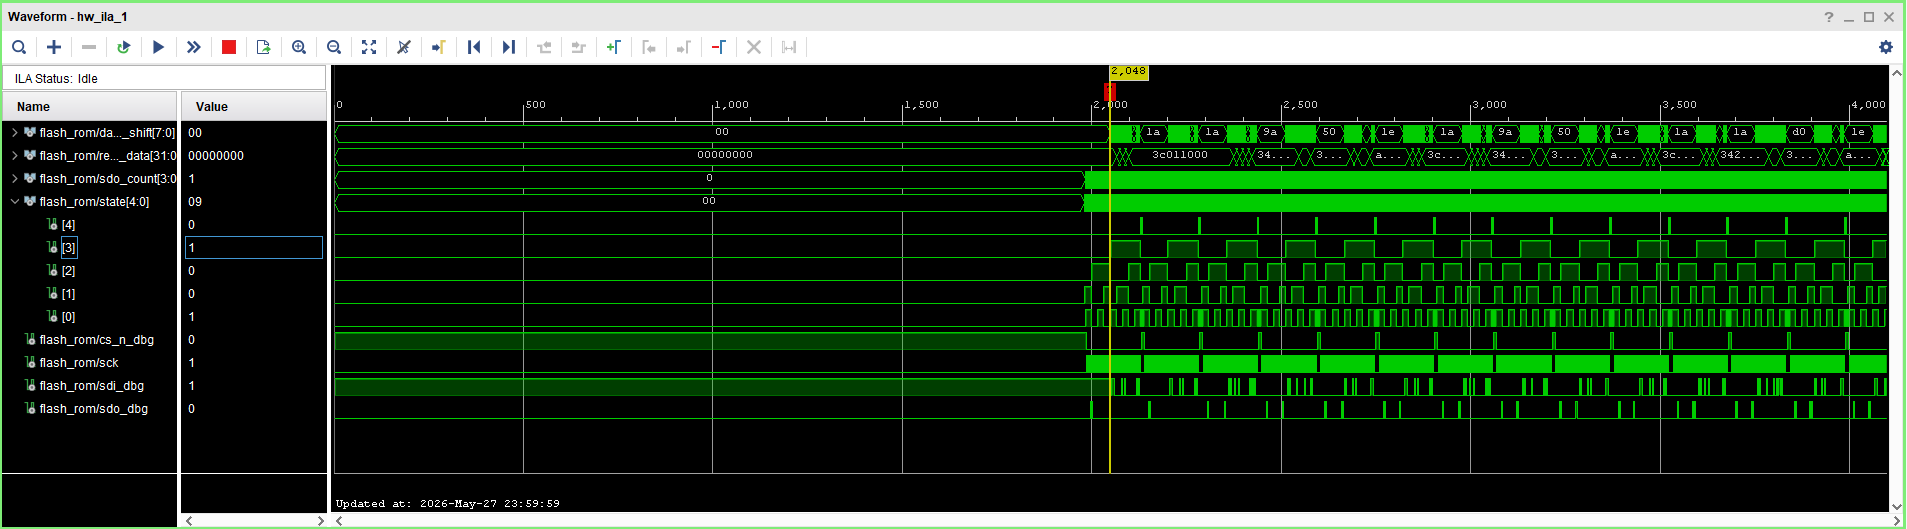
\includegraphics[width=0.9\textwidth]{img/ILA.png}
    \caption{ILA波形——\texttt{datain\_shift}逐拍累积至\texttt{0x3C}}
    \label{fig:ila}
\end{figure}

\textbf{调试经验}：本问题的调试过程经历了多轮纸上推导均未成功（even采样得到\texttt{0x78}，odd采样得到\texttt{0x1E}，两者恰好分别在正确值的两侧），最终通过ILA抓取\texttt{sck}、\texttt{sdi}、\texttt{sdo\_count}、\texttt{datain\_shift}、\texttt{state}等信号的实际波形，观察\texttt{datain\_shift}的逐拍变化序列（\texttt{00} $\to$ \texttt{01} $\to$ \texttt{02} $\to$ ... $\to$ \texttt{3c}），才精确定位了采样点偏差。这表明对于时序敏感的SPI接口设计，波形测量比纸上推导更可靠。
